\chapter{Laminar premixed flames}
\label{ch:premixed}

In a premixed flame fuel and oxidiser are mixed \emph{before} they burn (gas stove, Bunsen burner,
lean-premixed gas turbine). The flame is a thin front that propagates into the fresh mixture at a
speed set by the mixture itself, the \textbf{laminar burning velocity} $\SL$. Project Part~3 is
entirely about this object.

\section{The physical picture}

\begin{figure}[H]
\centering
\begin{tikzpicture}[xscale=1.6]
  \shade[left color=cold!15,right color=cold!15] (0,0) rectangle (2.6,2.4);
  \shade[left color=cold!15,right color=hot!40] (2.6,0) rectangle (3.6,2.4);
  \shade[left color=hot!40,right color=hot!25] (3.6,0) rectangle (7,2.4);
  \draw[very thick,hot] (3.6,0) -- (3.6,2.4);
  \draw[flow] (0.3,1.7) -- (1.3,1.7) node[above,pos=0.5,lbl] {$u_u=\SL$};
  \draw[flow,line width=2pt] (4.6,1.7) -- (6.6,1.7) node[above,pos=0.5,lbl] {$u_b=\SL\rho_u/\rho_b$};
  \draw[heat] (4.3,0.7) -- (3.0,0.7) node[below,pos=0.5,lbl] {heat};
  \draw[->,thick,derv,decorate,decoration={snake,amplitude=0.6mm,segment length=2mm}] (4.3,0.35) -- (3.0,0.35);
  \node[lbl,derv] at (2.3,0.35) {radicals};
  \node[lbl,align=center] at (1.3,0.8) {fresh mixture\\$T_u,\ \rho_u,\ Y_{k,u}$};
  \node[lbl,align=center] at (5.5,0.8) {burnt gas\\$T_b,\ \rho_b,\ Y_{k,b}$};
  \node[lbl,align=center,above] at (3.1,2.4) {preheat\\zone};
  \node[lbl,align=center,above] at (3.75,2.4) {reaction\\zone};
\end{tikzpicture}
\caption{A planar premixed flame in its own reference frame. Fresh gas arrives at $\SL$. Heat and
radicals diffuse \emph{upstream} from the reaction zone and preheat the incoming mixture until it
ignites. The burnt gas leaves faster because it has expanded.}
\label{fig:planar}
\end{figure}

\begin{intuition}
A premixed flame is a self-sustaining ignition wave. Each layer of fresh gas is heated by its
already-burning neighbour, ignites and in turn heats the next layer. The speed of this relay
depends on how fast heat diffuses ($\alpha$) and how fast the hot gas reacts ($\tau_{\rm chem}$).
That is why $\SL$ is a property of the mixture and not of the burner.
\end{intuition}

\section{Jump conditions across the flame}

\begin{derivation}[mass and momentum]
Steady and one-dimensional, \eqref{eq:mass} gives $\dd(\rho u)/\dd x=0$:
\begin{equation}
  \dot m\equiv\rho u=\rho_u\SL=\rho_bu_b=\text{const}
  \quad\Longrightarrow\quad
  \frac{u_b}{\SL}=\frac{\rho_u}{\rho_b}=\frac{T_b\,W_u}{T_u\,W_b}\approx 6\text{--}8 .
\end{equation}
Momentum: $\dot m\,\dd u/\dd x=-\dd p/\dd x$ (viscous terms cancel between the uniform ends), so
\[
p_u-p_b=\dot m\,(u_b-u_u)=\rho_u\SL^2\Big(\frac{\rho_u}{\rho_b}-1\Big)\approx 1.2\times0.4^2\times6\approx\SI{1}{\pascal}.
\]
The pressure drop is negligible compared with \SI{101325}{\pascal}, which justifies the low-Mach
approximation (\secref{sec:lowmach}).
\end{derivation}

\section{The 1D flame equations}
\label{sec:1deqs}

Steady, 1D, low-Mach versions of \eqref{eq:species} and \eqref{eq:temperature}, with $j_k=\rho Y_kV_k$:
\begin{align}
  \dot m\od{Y_k}{x}&=-\od{j_k}{x}+W_k\wdot_k ,\label{eq:1dY}\\
  \dot m\,c_p\od{T}{x}&=\od{}{x}\Big(\lambda\od{T}{x}\Big)-\Big(\sum_kj_kc_{p,k}\Big)\od{T}{x}-\sum_kh_kW_k\wdot_k .\label{eq:1dT}
\end{align}
Boundary conditions: fresh state ($T_u$, $Y_{k,u}$) far upstream and zero gradients far downstream.

\begin{keypoint}[$\SL$ is an eigenvalue]
The equations are invariant under a shift $x\to x+c$, so the flame can sit anywhere. To get a
unique solution one extra condition is imposed: Cantera fixes the temperature at one grid point.
In exchange, $\dot m$ is no longer prescribed but \emph{computed}. The flame ``chooses'' its own
mass flux, and $\SL=\dot m/\rho_u=$ \code{flame.velocity[0]}.
\end{keypoint}

\section{The burnt state is the HP equilibrium}
\label{sec:burntHP}

\begin{derivation}[for any Lewis numbers]
Write the enthalpy form \eqref{eq:enthalpy} in 1D (low Mach, no viscous heating):
$\dot m\,\dd h/\dd x=-\dd q/\dd x$ with $q=-\lambda\,\dd T/\dd x+\sum_kh_kj_k$. Hence
\[
\od{}{x}\Big[\dot m\,h+q\Big]=0\quad\Longrightarrow\quad \dot m\,h+q=\text{const}.
\]
Far upstream and far downstream all gradients and diffusive fluxes vanish ($q=0$), so
$h_b=h_u$. The same argument applied to each \emph{element} (chemistry does not create atoms)
gives equal elemental composition at both ends. Far downstream the gas is also no longer
changing, i.e.\ it is at chemical equilibrium. A state with the same $h$, $p$ and elements that is at
equilibrium is precisely \code{equilibrate("HP")} of the fresh gas.
\end{derivation}

\begin{warning}[why the end of your domain is \emph{not} that state]
Recombination of radicals and, for hydrocarbons, oxidation of CO are slow. In a domain a few
centimetres long, the gas leaving at \code{flame.T[-1]} may still be measurably short of
equilibrium (\figref{fig:grid}). Also, a coarse grid gives an error in the burnt state. Hence the
project's rule: \textbf{compare the end state with HP equilibrium; if the deviation is above 1\%,
refine; and quote $\Tad$ from equilibrium, not from \code{flame.T[-1]}}.
\end{warning}

\section{Flame structure}

\begin{figure}[H]
\centering
\begin{tikzpicture}[xscale=1.5,yscale=1.0]
  \draw[->] (-3.2,0) -- (4.2,0) node[right] {$x$};
  \draw[very thick,hot,domain=-3:0,samples=60] plot (\x,{0.4+3.1*exp(1.6*\x)});
  \draw[very thick,hot,domain=0:4,samples=20] plot (\x,{3.5+0.15*(1-exp(-\x))});
  \node[hot,right] at (4,3.7) {$T$};
  \draw[very thick,cold,domain=-3:0,samples=60] plot (\x,{3.0-2.75*exp(1.6*\x)});
  \draw[very thick,cold,domain=0:0.5,samples=20] plot (\x,{0.25*(1-\x/0.5)});
  \node[cold,left] at (-3,3.0) {$Y_F$};
  \fill[keyc!40,opacity=0.7,domain=-0.6:0.6,samples=60] plot (\x,{2.6*exp(-12*\x*\x)}) -- cycle;
  \node[keyc!60!black] at (0.9,2.3) {$\dot q$};
  \draw[dashed] (-0.3,-0.2) -- (-0.3,4.1);
  \draw[dashed] (0.3,-0.2) -- (0.3,4.1);
  \draw[<->] (-3,4.3) -- (-0.3,4.3) node[midway,above,lbl] {preheat: convection $\approx$ diffusion};
  \draw[<->] (0.3,4.3) -- (4,4.3) node[midway,above,lbl] {post-flame: slow recombination};
  \node[lbl,align=center] at (0,-0.6) {reaction zone\\ $\sim\delta_L/\beta$};
\end{tikzpicture}
\caption{Classical three-zone structure. In the preheat zone chemistry is negligible and the
profile is exponential. The thin reaction zone is where almost all heat is released. Downstream,
slow recombination brings the gas to equilibrium.}
\label{fig:zones}
\end{figure}

\begin{derivation}[preheat zone profile]
Upstream of the reaction zone $\wdot_k\approx0$. With constant properties, \eqref{eq:1dT}
becomes $\dot mc_p\,T'=\lambda T''$, or $\SL T'=\alpha_u T''$. The solution that tends to $T_u$ at
$-\infty$ is
\begin{equation}
  T-T_u=(T_r-T_u)\,\exp\!\Big(\frac{\SL\,x}{\alpha_u}\Big),
\end{equation}
where $T_r$ is the temperature where reaction starts. The e-folding length is the
\textbf{diffusive flame thickness} $\delta_d=\alpha_u/\SL$.
\end{derivation}

\begin{figure}[H]
\centering
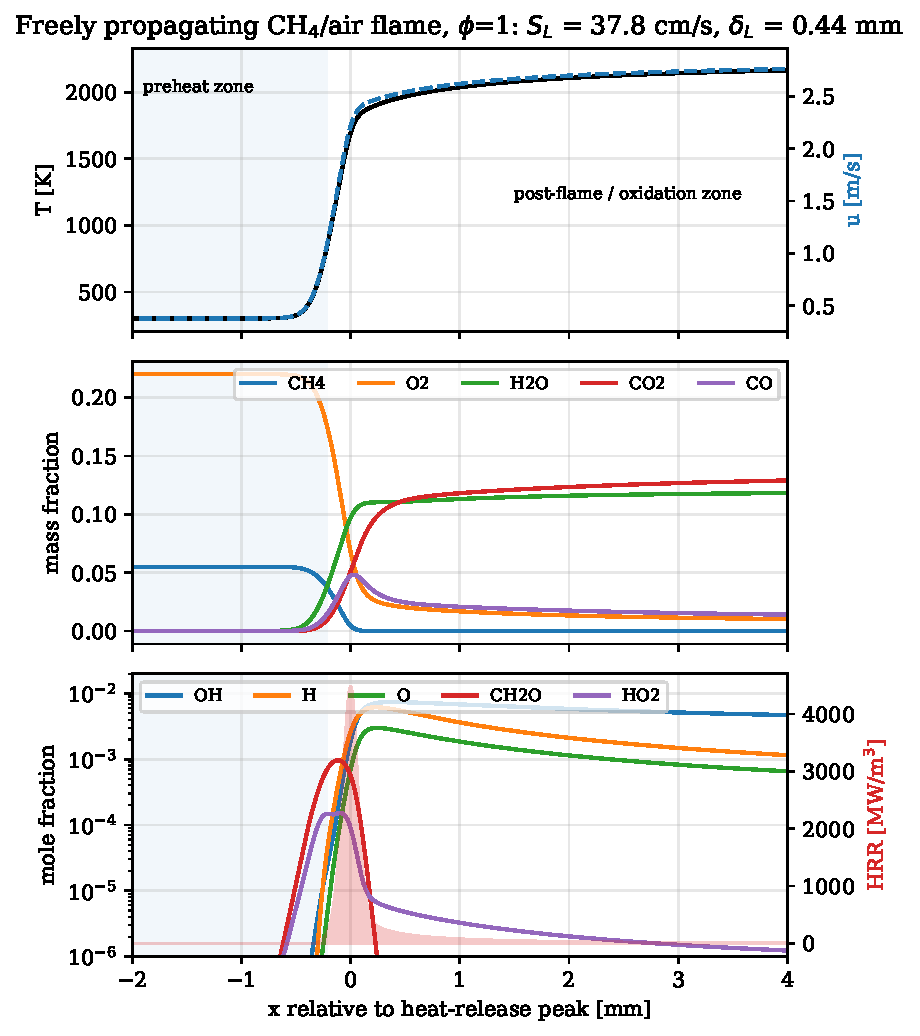
\includegraphics[width=0.85\textwidth]{freeflame_ch4}
\caption{Computed stoichiometric \ce{CH_4}/air flame (GRI-Mech 3.0, mixture-averaged). Top: $T$ and
$u$; the gas accelerates by $\rho_u/\rho_b$. Middle: major species. Bottom: radicals and the heat
release rate (shaded). Note that HRR peaks where $T$ is still rising. Intermediates such as
\ce{CH_2O} and \ce{HO_2} appear upstream of the HRR peak, and H, O, OH spill into the burnt gas
and decay slowly.}
\label{fig:ffch4}
\end{figure}

\section{How fast and how thick: scaling laws}
\label{sec:scaling}

\begin{derivation}[Mallard--Le~Chatelier / Zeldovich scaling]
Balance the three terms of \eqref{eq:1dT} over a flame of thickness $\delta$ and temperature rise
$\Delta T=T_b-T_u$:
\[
\underbrace{\rho_u\SL c_p\frac{\Delta T}{\delta}}_{\text{convection}}\sim
\underbrace{\lambda\frac{\Delta T}{\delta^2}}_{\text{diffusion}}\sim
\underbrace{\dot q}_{\text{reaction}} .
\]
Convection $\sim$ diffusion gives $\delta\sim\alpha/\SL$. Diffusion $\sim$ reaction gives
$\delta^2\sim\alpha\tau_c$ with chemical time $\tau_c=\rho c_p\Delta T/\dot q$. Eliminating $\delta$:
\begin{equation}
  \boxed{\SL\sim\sqrt{\frac{\alpha}{\tau_c}},\qquad \delta\sim\frac{\alpha}{\SL}\sim\sqrt{\alpha\tau_c},\qquad
  \frac{\SL\,\delta}{\alpha}\sim1 .}
  \label{eq:SLscaling}
\end{equation}
\end{derivation}

\begin{intuition}
A flame is as thick as heat can diffuse in one chemical time, and travels one thickness per
chemical time. Fast chemistry gives fast, thin flames. More diffusive mixtures (\ce{H_2}) give faster,
thicker ones. The product $\SL\delta$ is set by diffusivity alone: the \textbf{flame Péclet number}
$\SL\delta/\alpha_u$ is a near-universal constant.
\end{intuition}

\paragraph{Temperature sensitivity.} Reaction happens near $T_b$, where
$\dot q\propto e^{-E/\Ru T_b}$, so
\begin{equation}
  \SL\propto\exp\!\Big(-\frac{E}{2\Ru T_b}\Big).
\end{equation}
The flame speed follows the burnt temperature, exponentially. Anything that raises $T_b$
(stoichiometry near the $\Tad$ peak, preheating) raises $\SL$ strongly. The
\textbf{Zeldovich number} $\beta=E(T_b-T_u)/(\Ru T_b^2)\approx8$--$12$ measures this sensitivity.
The reaction zone is thinner than the flame by a factor $\sim\beta$.

\paragraph{Pressure dependence.}
\begin{derivation}[$\SL\propto p^{n/2-1}$]
From \chapref{ch:transport}, $\alpha\propto1/p$. For a global reaction of overall order $n$
(\secref{sec:global}), $\dot q\propto p^n$, while $\rho c_p\Delta T\propto p$, so $\tau_c\propto p^{1-n}$. Then
\[
\SL\propto\sqrt{p^{-1}\,p^{\,n-1}}=p^{\,n/2-1},\qquad
\delta\propto\frac{\alpha}{\SL}\propto p^{-n/2}.
\]
For a bimolecular reaction ($n=2$), $\SL$ would be pressure-independent. Measured exponents are
\emph{negative} because three-body termination (R5) grows faster with pressure than branching,
which lowers the effective order below 2. Note also that $\SL\delta\propto\alpha\propto1/p$: the
product is \emph{not} constant with pressure, but the Péclet number $\SL\delta/\alpha_u$ is.
\end{derivation}

\paragraph{Preheat.} Raising $T_u$ raises $T_b$ (\secref{sec:Tad}) and $\alpha$. Empirically
$\SL\propto T_u^m$ with $m\approx1.5$--$2$ for hydrocarbons. A common correlation is
$\SL=\SL^0(T_u/T_0)^{m}(p/p_0)^{n_p}$, fitted separately for each $\phi$.

\section{Thickness definitions}

\begin{itemize}
  \item \textbf{Thermal thickness} (used in the project):
        \begin{equation}
          \delta_L=\frac{T_b-T_u}{\max|\dd T/\dd x|} .
        \end{equation}
        Robust and easy to measure: draw the tangent at the steepest point.
  \item \textbf{Diffusive thickness} $\delta_d=\alpha_u/\SL$. It is much smaller (5--7$\times$,
        \figref{fig:SLphi}), because $\alpha$ is evaluated in the cold gas while the gradient sits where the gas
        is hot and far more diffusive. Blint's correlation $\delta_L\approx2\delta_d(T_b/T_u)^{0.7}$
        accounts for this.
\end{itemize}

\begin{figure}[H]
\centering
\begin{tikzpicture}[xscale=1.3,yscale=0.9]
  \draw[->] (-2.5,0) -- (3,0) node[right] {$x$};
  \draw[->] (-2.5,0) -- (-2.5,3.6) node[above] {$T$};
  \draw[very thick,hot,domain=-2.4:2.8,samples=80] plot (\x,{0.4+2.6/(1+exp(-2.4*\x))});
  \draw[dashed] (-2.5,0.4) -- (2.8,0.4) node[right,lbl] {$T_u$};
  \draw[dashed] (-2.5,3.0) -- (2.8,3.0) node[right,lbl] {$T_b$};
  \draw[thick,keyc] (-0.83,0.4) -- (0.83,3.0);
  \draw[<->,keyc] (-0.83,0.15) -- (0.83,0.15) node[midway,below,lbl] {$\delta_L$};
  \node[lbl,keyc,align=left] at (1.9,1.4) {tangent at\\max slope};
\end{tikzpicture}
\caption{Thermal thickness: the width of the tangent at the inflexion point between $T_u$ and $T_b$.}
\end{figure}

\section{Two definitions of flame speed}

\begin{derivation}[consumption speed]
Integrate the fuel equation \eqref{eq:1dY} over the whole domain. The diffusive flux vanishes at both
ends:
\[
\dot m\,(Y_{F,b}-Y_{F,u})=\int_{-\infty}^{\infty}W_F\wdot_F\,\dd x
\quad\Longrightarrow\quad
S_c=\frac{-\int W_F\wdot_F\,\dd x}{\rho_u\,(Y_{F,u}-Y_{F,b})}.
\]
\end{derivation}
\begin{itemize}
  \item \textbf{Displacement speed} $S_u$: the velocity of the fresh gas relative to the flame front
        (\code{flame.velocity[0]} in a free flame). Depends on the frame and on stretch.
  \item \textbf{Consumption speed} $S_c$: how fast fuel is actually consumed per unit flame area.
        Robust in stretched or curved flames.
\end{itemize}
For a planar, unstretched, adiabatic flame they are identical, and a good check of your solution.

\section{Measuring $\SL$: the Bunsen flame}

\begin{figure}[H]
\centering
\begin{tikzpicture}
  \draw[thick] (-0.8,-1.5) -- (-0.8,0); \draw[thick] (0.8,-1.5) -- (0.8,0);
  \draw[very thick,hot] (-0.8,0) -- (0,2.8) -- (0.8,0);
  \draw[flow] (0,-1.3) -- (0,-0.3) node[midway,left,lbl] {$U$};
  \draw[flow] (-0.3,1.2) -- ++(0,0.9);
  \draw[->,thick,keyc] (-0.4,1.4) -- ++(-0.62,0.18) node[left,lbl] {$\SL$};
  \draw (0,2.8) -- (0,1.9); \draw (0,2.2) arc (-90:-106:0.6) node[below left,lbl] {$\alpha$};
  \node[lbl,align=left] at (3.4,1.2) {Normal velocity component\\balances flame speed:\\[2pt]
       $\SL=U\sin\alpha$};
\end{tikzpicture}
\caption{The flame cone settles where the component of the jet velocity normal to the front
equals $\SL$. Historically the main experimental method. Today counterflow and spherical-flame
methods with stretch correction are preferred.}
\end{figure}

\section{Dependence on equivalence ratio}

\begin{figure}[H]
\centering
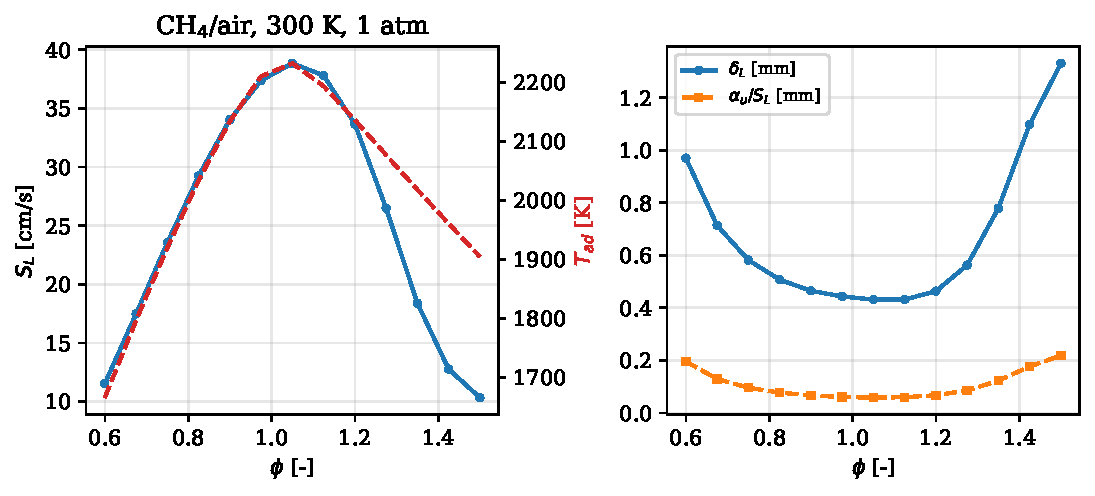
\includegraphics[width=\textwidth]{SL_phi_ch4}
\caption{Left: computed \ce{CH_4}/air flame speed (blue) and $\Tad$ (red). $\SL$ follows $\Tad$
but falls much faster away from the peak: the exponential temperature sensitivity of
\secref{sec:scaling}. Right: thermal thickness $\delta_L$ and $\alpha_u/\SL$. Slow flames are thick.}
\label{fig:SLphi}
\end{figure}

\begin{intuition}[what moves the $\SL$ peak]
For \ce{CH_4}/air, the $\SL$ peak sits near the $\Tad$ peak. For other fuels the two can separate
far apart, because $\SL\sim\sqrt{\alpha/\tau_c}$ depends not only on $T_b$ but also on
\begin{itemize}
  \item the \emph{diffusivity} of the mixture, which grows with the fraction of a light fuel;
  \item the \emph{radical pool}: how much H the reaction zone can produce and back-diffuse;
  \item which reactant is deficient and how fast \emph{it} diffuses.
\end{itemize}
In Part~3, Task~4 you compare the $\SL(\phi)$ peak of \ce{H_2} with the $\Tad(\phi)$ peak from Part~1.
Use these three items to explain the difference.
\end{intuition}

\section{Lewis-number and preferential-diffusion effects}
\label{sec:lepremixed}

Under unity Lewis number (\secref{sec:unityLe}) enthalpy and element ratios are constant through
the flame. Every point inside the flame has the fresh-gas $\phi$ and enthalpy. With real
transport and a light fuel:
\begin{itemize}
  \item \textbf{\ce{H_2} runs ahead.} In the preheat zone \ce{H_2} diffuses towards the reaction zone
        faster than heat diffuses out. The local element ratio changes, so a mixture fraction based on
        H atoms is \emph{not} constant across the flame (Part~3, Task~3c).
  \item \textbf{H atoms run back.} The H radical ($\mathrm{Le}\approx0.2$) diffuses far upstream into
        the cool preheat zone and starts the chain there. Forcing $D_{\rm H}=\alpha$ suppresses this.
  \item \textbf{Local enthalpy deviates.} Inside the flame $h$ can be above or below $h_u$ even
        though both ends are equal (\secref{sec:burntHP}).
\end{itemize}

\begin{figure}[H]
\centering
\begin{tikzpicture}[xscale=1.4,yscale=1.0]
  \draw[->] (-3,0) -- (3.4,0) node[right] {$x$};
  \draw[->] (-3,0) -- (-3,2.6) node[above] {$Z$};
  \draw[thick,dashed,gray] (-3,1.2) -- (3.2,1.2) node[right,lbl] {$\mathrm{Le}=1$: $Z=Z_u$};
  \draw[very thick,intu,domain=-3:3.2,samples=80] plot (\x,{1.2+0.8*exp(-1.5*(\x-0.1)*(\x-0.1))});
  \node[intu,lbl] at (1.6,2.1) {mixture-averaged};
  \draw[dotted] (0.3,0) -- (0.3,2.4) node[above,lbl] {reaction zone};
\end{tikzpicture}
\caption{Qualitative sketch: with $\mathrm{Le}_{\ce{H_2}}<1$, an H-element-based mixture fraction
bulges inside the flame and returns to the fresh value downstream. Its shape, size and sign
depend on $\phi$. Measuring them is your task.}
\end{figure}

\paragraph{Stretch.} Real flames are curved and strained. With $\mathrm{Le}<1$ a stretched lean flame
burns \emph{faster}, which leads to cellular instabilities in lean \ce{H_2} flames. The planar flame of the
project is unstretched, the reference case to which stretch effects are compared through
Markstein numbers.

\section{Solving a free flame in Cantera}

\begin{lstlisting}
gas = ct.Solution("gri30.yaml")
gas.set_equivalence_ratio(1.0, "CH4", "O2:1, N2:3.76")
gas.TP = 300.0, ct.one_atm

flame = ct.FreeFlame(gas, width=0.03)            # domain [m]: ~50-100 flame thicknesses
flame.transport_model = "mixture-averaged"
flame.set_refine_criteria(ratio=2, slope=0.05, curve=0.1)
flame.set_max_grid_points(flame.flame, 10000)
flame.solve(loglevel=0, auto=True)               # auto: robust initial-guess strategy

S_L = flame.velocity[0]                          # [m/s]
dTdx = np.gradient(flame.T, flame.grid)
delta_L = (flame.T[-1] - flame.T[0]) / dTdx.max()
hrr = flame.heat_release_rate                    # [W/m^3]
\end{lstlisting}

\begin{figure}[H]
\centering
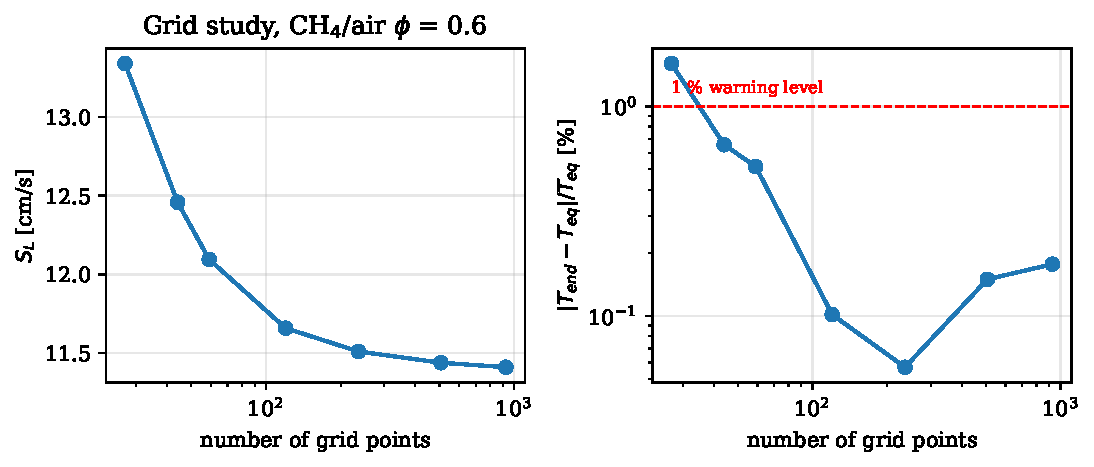
\includegraphics[width=\textwidth]{grid_convergence}
\caption{Grid study of a lean ($\phi=0.6$) \ce{CH_4} flame. The coarsest grid (27 points, close to
the default) over-predicts $\SL$ by 17\%. The burnt-temperature error falls with refinement until it
reaches a floor set by the finite domain (slow CO oxidation), not by the grid. That floor is why
$\Tad$ must come from equilibrium.}
\label{fig:grid}
\end{figure}

\begin{project}[Part 3]
\begin{itemize}
  \item Task 1: three panels against $x$ in mm. Ask yourself why the HRR peak precedes the $T$ maximum
        (\figref{fig:ffch4}), and where the radicals are made versus where they survive.
  \item Task 2: the equilibrium check is \secref{sec:burntHP}. Remember the warning above.
  \item Task 3: transport comparison, see \secref{sec:lepremixed}. For a fair temperature comparison, shift each
        profile so that $T=(T_u+T_b)/2$ sits at $x=0$.
  \item Task 4: sweep $\phi$ from a converged neighbour (\secref{sec:ct-sweeps}). Check $\SL\delta_L/\alpha_u$
        against \eqref{eq:SLscaling}.
  \item Task 5: fit $\ln\SL$ vs $\ln p$ and vs $\ln T_u$ by linear regression (\code{np.polyfit}). Compare your
        exponent with $n/2-1$ and decide what effective order $n$ it implies.
\end{itemize}
\end{project}

\begin{selfcheck}
\begin{enumerate}
  \item Why must \code{flame.velocity[-1]/flame.velocity[0]} equal $\rho_u/\rho_b$?
  \item If the domain is too short, which boundary condition is violated and what happens to $\SL$?
  \item A mechanism over-predicts $\Tad$ by \SI{30}{\kelvin}. Using $\SL\propto e^{-E/2\Ru T_b}$ with
        $E/\Ru=\SI{20000}{\kelvin}$ and $T_b=\SI{2200}{\kelvin}$, by how much does it over-predict $\SL$?
\end{enumerate}
\end{selfcheck}
